\section{Resource usage}

A further test was conducted to measure the CPU usage of the device running the pipeline.
GPU usage was not measured, since the value would spike to 100\% as soon as there was any task running on the GPU: the values would therefore not be indicative of whether other computations could be performed at the same time.
The CPU results are shown in figure~\ref{fig:usage}.

In the Jetson Orin Nano, all CPU cores spend the full processing time standing at almost 100\%, indicating that all resources of the device are devolved to the task.
On the Jetson AGX Xavier, the situation is slightly different: the most notable fact is that the bottleneck shifts from the \locate* step to the \match*, and the overall processing speed is lower.
This is visible in the graph as a sudden de-loading of the device: when all steps are running, the full device is in use; after the \locate* finishes processing all the video, some cores reduce their usage.
This may be an indication that, being a more premium device, the Xavier is faster than the Orin at transferring data to the RAM; however the fact of being older penalizes it on CPU computational speed.

\begin{figure}
	\centering
	\minipage{0.5\textwidth}
	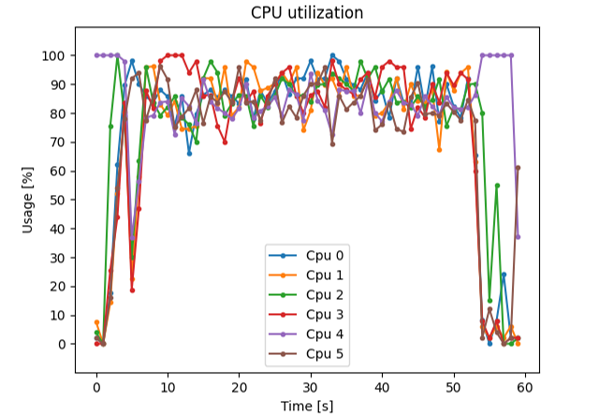
\includegraphics[width=\linewidth]{images/speed/usage-orin.png}
	\caption*{(a)}
	\endminipage\hfill
	\minipage{0.5\textwidth}
	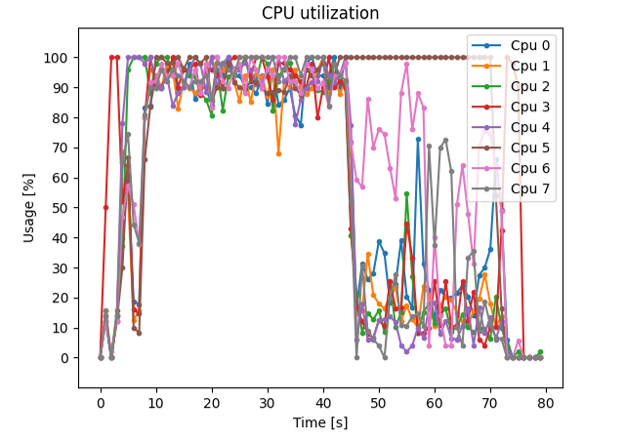
\includegraphics[width=\linewidth]{images/speed/usage-xavier.png}
	\caption*{(b)}
	\endminipage

	\captionsetup{list=true}

	\caption{\centering CPU usage per core, while running the pipeline on (a) the Jetson Orin Nano and (b) the Jetson AGX Xavier}\label{fig:usage}
\end{figure}
